\documentclass[12pt, accentcolor=tud1b]{tudreport}
\usepackage{hyperref}
\usepackage{graphicx}
\usepackage{color}
%\usepackage{ngerman}
%Gummi|065|=)
\title{\textbf{Anise GUI Tutorial}}
\subtitle{Artur Fast \\ Frederik L\"uhrs \\ Mehrad Mohammadian \\ Tobias Lippert}

\institution{Department of Computer Science \\  Bachelor Lab WS14/15 \\ March 31, 2015}

\begin{document}
\maketitle
\noindent
This tutorial is to show you how to work with the \emph{Anise GUI}. It is all about creating networks
(meshes) of nodes and simulating your results with the \emph{Anise Framework}.

\section*{Getting started}
\begin{minipage}{0.5\textwidth}
When you start the GUI for the first time you will
have to select a Anise executable from your file
system. You can skip this by clicking \emph{Ignore}.\\
This is not recommended because you will not be
able to create meshes without a framework
executable. \\
You can change the executable later on ("\emph{Properties}"  --\textgreater{} "\emph{Select Framework Executable}"). \\ \\
The GUI has to restart afterwards.
\end{minipage}
\begin{minipage}{0.5\textwidth}
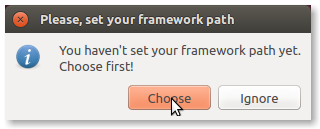
\includegraphics[width=\textwidth]{choose_path}
\end{minipage}

\section*{Loading a file}
If have previously saved or self-written JSON files you want to load to the GUI you can do this by choosing "load" form the file menu. You can also use the short cut \emph{CTRL + L}.

\section*{Create own meshes}
You can create your own meshes by simply dragging nodes from the catalog on the top into the editing area in the center. 
\begin{center}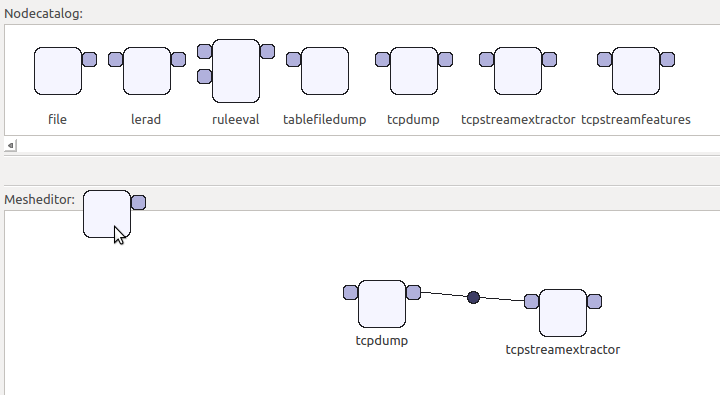
\includegraphics[width=0.9\textwidth]{add_node_cut}\end{center}
\newpage

\section*{Adding connections}
You can create connections between nodes by clicking on an output gate (right side of a node).\\
You automatically enter the connection mode. All possible destinations you can draw a connection to
will be highlighted in green. \\
If you want to add joints to your connection click on the spot the joint
should be placed. To exit connection mode without creating a connection right-click anywhere.
\begin{center}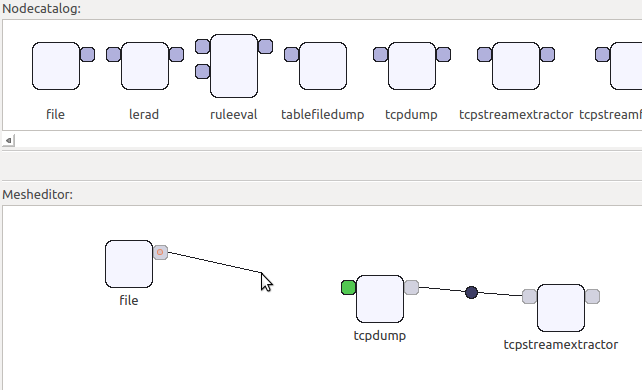
\includegraphics[width=0.9\textwidth]{draw_connection_cut}\end{center}

\section*{Editing node parameters}

\begin{minipage}{0.5\textwidth}
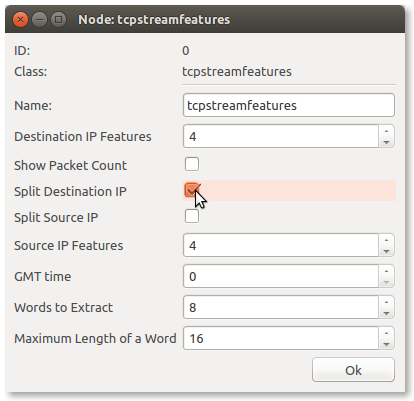
\includegraphics[width=\textwidth]{edit_window_cut}
\end{minipage}
\begin{minipage}[t]{0.5\textwidth}\vspace{-120pt}For editing node parameters doubleclick a node. A window opens showing you all the parameters and their values. \end{minipage}\newpage \noindent
It is also possible to eidt parameters using the property table. You will have to enable the "\emph{Show Details}" option in the top right corner.

\begin{center}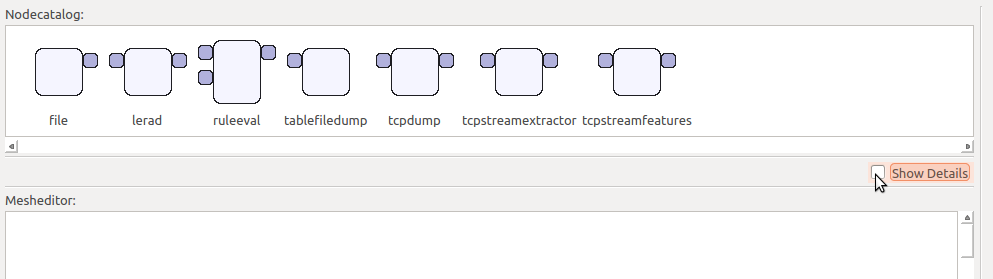
\includegraphics[width=0.9\textwidth]{uncheck_details_cut}\end{center}
\noindent
When you now select a node, its description, name, parameters and further information will be
shown on the right side. You can edit the parameters and the node's name.
\begin{center}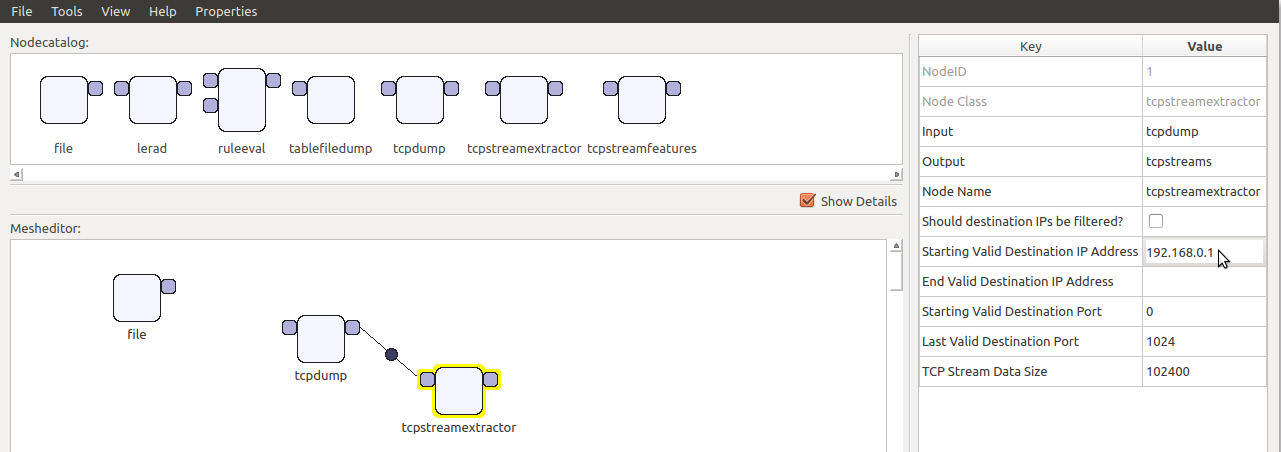
\includegraphics[width=0.9\textwidth]{change_parameters_cut}\end{center} 
\noindent \\ \\
If "\emph{Show Details}" is checked, all relevant information about the nodes inside the catalog will also
be shown on the right side by clicking on them.
\begin{center}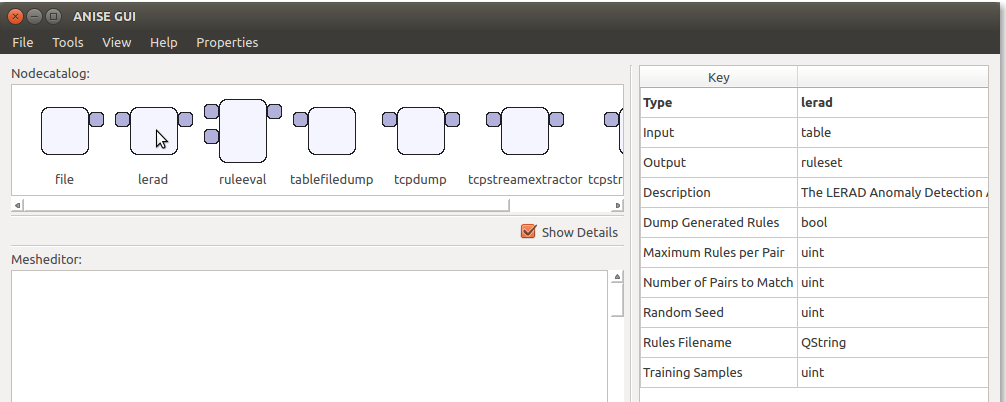
\includegraphics[width=0.9\textwidth]{type_info_cut}\end{center} 
\newpage

\section*{Simulation}
Before you execute your mesh you will have to save it.
Start the simulation with "\emph{Tools}" --> "\emph{Start Simulation}" or use \emph{CTRL + R}. \\ \\
Every node has three states: \textbf{
\begin{itemize}\itemsep0pt
\item {\color{green}idle}
\item {\color{gray}initializing}
\item {\color{blue}procressing}
\end{itemize}}
	\begin{minipage}{0.5\textwidth}
	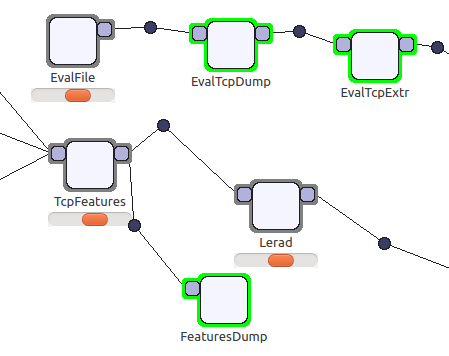
\includegraphics[width=\textwidth]{sim_start_cut}
	\end{minipage}
	\hfill
	\begin{minipage}{0.45\textwidth}
	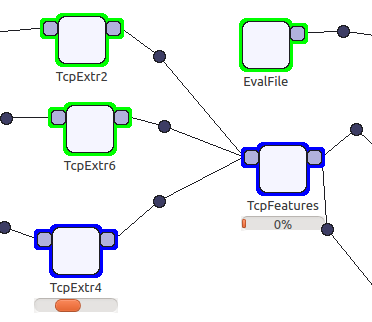
\includegraphics[width=\textwidth]{on_run_cut}
	\end{minipage}

\end{document}
